\documentclass[12pt,a4paper]{article}

%\usepackage[ngerman]{babel}
\usepackage[utf8x]{inputenc}
\usepackage[T1]{fontenc}

%\usepackage[hyphens]{url}
\usepackage{pbox}
\usepackage{float}
\usepackage[breaklinks]{hyperref}
\usepackage[hyphenbreaks]{breakurl}
\usepackage{breakurl}
\usepackage{placeins}
\usepackage{wrapfig}
\usepackage{rotating}
\usepackage{titlesec}
\usepackage{hvfloat}
\usepackage{lipsum}
\usepackage{palatino}
\usepackage{a4wide}
\usepackage{multicol}
\usepackage{float}
\usepackage{graphicx}
\usepackage{amsfonts}
\usepackage{amsmath}
\usepackage{mathtools}
\usepackage{amsthm}
\usepackage{amssymb}
\usepackage{array}
\usepackage{listings}
\usepackage{colortbl}
\usepackage{endnotes}
\usepackage{inconsolata}
\usepackage{epstopdf}
\usepackage{blindtext}
\usepackage{color}
\usepackage{pdflscape}
\usepackage{capt-of}
\usepackage{sidecap}
\usepackage[usenames,dvipsnames]{xcolor}
\usepackage{tikzsymbols}
\usepackage{phaistos}
\usepackage{bbding}
\usepackage[francais,english,german]{babel}
%\usepackage{fontawesome}
%\usepackage[small,compact]{titlesec}
\usepackage{tikz}
%\usetikzlibrary{arrows,automata}

\definecolor{light-gray}{gray}{0.95}

\usepackage{booktabs}                   %gives \toprule, \midrule and \bottomrule for professional looking tables
\usepackage{fixltx2e}                   %fixltx2e adds \textsubscript{}, textsubscript should already be there
\usepackage{threeparttable}             %Provides notes in tables (in addition to the caption)
\usepackage{tabularx}                   %Defines column type X for tables with auto linebreaks. For REALLY big tables use one of the more specialized packages
\usepackage{caption}
%\usepackage{subcaption}
%\captionsetup{margin=0.8cm,aboveskip=8mm,labelfont=bf,labelformat=simple,labelsep=period,textfont=small}
% \setcounter{tocdepth}{2}        %Two should be default anyway
% \setlength{\parskip}{1ex plus 0.5ex minus 0.5ex}        %Space of a paragraph, note the variability, gives latex more room for optimization
\titlespacing{\section}{0pt}{20pt}{16pt}
\titlespacing{\subsection}{0pt}{20pt}{16pt}
\titlespacing{\subsubsection}{0pt}{20pt}{16pt}
\setlength{\parindent}{0pt}       %Basically a whole lot of \noindents before every paragraph ;)
\usepackage{nicefrac}                   %fraction style (a/b) use with \nicefrac{}{}
% \setlength{\headheight}{15pt}
% \usepackage{emptypage}          %Empty pages are really empty, no header or anything

\lstset{
 language=AWK,                % choose the language of the code
 basicstyle=\footnotesize,       % the size of the fonts that are used for the code
 numbers=left,                   % where to put the line-numbers
 numberstyle=\footnotesize,      % the size of the fonts that are used for the line-numbers
 stepnumber=1,                   % the step between two line-numbers. If it is 1 each line will be numbered
 numbersep=10pt,                  % how far the line-numbers are from the code
 showspaces=false,               % show spaces adding particular underscores
 showtabs=false,                 % show tabs within strings adding particular underscores
 frame=single,   		% adds a frame around the code
 tabsize=4,  		% sets default tabsize to 2 spaces
 captionpos=t,   		% sets the caption-position to bottom
 breaklines=true,    	% sets automatic line breaking
 breakatwhitespace=false,    % sets if automatic breaks should only happen at whitespace
 showstringspaces=false,
 mathescape=false,		%allo entering math environment
 backgroundcolor=\color{light-gray},
 morekeywords={init, par, foreach, return, min, allocate, abs, delete, is_member, insert},            % if you want to add more keywords to the set
 keywordstyle=\color{blue},          % keyword style
 commentstyle=\color{OliveGreen},       % comment style
 stringstyle=\color{orange}
}

\hypersetup{
    bookmarks=true,         % show bookmarks bar?
    unicode=true,          % non-Latin characters in Acrobat’s bookmarks
    pdftoolbar=true,        % show Acrobat’s toolbar?
    pdfmenubar=true,        % show Acrobat’s menu?
    pdffitwindow=false,     % window fit to page when opened
    pdfstartview={Fit},    % fits the width of the page to the window
    pdftitle={Homework 2:  Modélisation des écosystèmes aquatiques - Nicolas Piret et Yann Sp\"ori},    % title
    pdfauthor={Nicolas Piret et Yann Sp\"ori},     % author
    %pdfsubject={Subject},   % subject of the document
    %pdfcreator={Creator},   % creator of the document
    %pdfproducer={Producer}, % producer of the document
    %pdfkeywords={keywords}, % list of keywords
    pdfnewwindow=true,      % links in new window
    colorlinks=false,       % false: boxed links; true: colored links
    linkcolor=red,          % color of internal links
    citecolor=green,        % color of links to bibliography
    filecolor=magenta,      % color of file links
    urlcolor=cyan           % color of external links
}

\newcommand{\citeme}[1]{\Large\textsuperscript{\textbf{\textcolor{Blue}{cite me!}(#1)}}\normalsize}
\newcommand{\todo}{\textbf{\textcolor{red}{ TODO! }}}
\newcommand{\refer}[1]{\ref{#1}~(page~\pageref{#1})}
\newcommand{\al}[0]{$\alpha$}
\newcommand{\alimp}[0]{$\alpha$\,IMP\ }
\newcommand{\alimps}[0]{$\alpha$\,IMPs\ }   %These are not nice, could have used sth like \al-IMPs or {\alimp}s
\newcommand{\be}[0]{$\beta$}
\newcommand{\beimp}[0]{$\beta$\,IMP\ }
\newcommand{\beimps}[0]{$\beta$\,IMPs\ }
\newcommand{\supp}[0]{Supplementary Material\ }
\newcommand{\angs}[0]{\,\AA}
\newcommand{\method}[1]{\textbf{#1}}
\newcommand{\ie}[0]{\textit{i.e.\ }}
\newcommand{\eg}[0]{e.g.\ }
\newcommand{\cf}[0]{cf.\ }
\newcommand{\chap}[0]{cp.\ }
\newcommand{\dbid}[1]{{\fontfamily{phv}\selectfont\footnotesize\lowercase{#1}}}   
\newcommand{\figintro}[1]{\textbf{#1}}
\newcommand\abs[1]{\left|#1\right|}
\newcommand{\highlight}[1]{%
  \colorbox{yellow!50}{$\displaystyle#1$}}
\newcommand{\highlightgreen}[1]{%
  \colorbox{green!50}{$\displaystyle#1$}}
\newcommand{\hr}[0]{
\par{
\noindent\makebox[\linewidth]{\rule{\textwidth}{1pt}}
}
}

\usepackage[sort&compress,comma,numbers]{natbib}

% table of contents
\renewcommand{\contentsname}{Table of contents}

% Bibliography
\usepackage[numbib,notlof,notlot,nottoc,section]{tocbibind}
\renewcommand\tocbibname{References}

\setcounter{secnumdepth}{4}

\titleformat{\paragraph}
{\normalfont\normalsize\bfseries}{\theparagraph}{1em}{}
\titlespacing*{\paragraph}
{0pt}{3.25ex plus 1ex minus .2ex}{1.5ex plus .2ex}

\usepackage{xcolor}
\definecolor{c0}{Hsb}{000,1.0,0.5}
\definecolor{c1}{Hsb}{024,1.0,0.5}
\definecolor{c2}{Hsb}{048,1.0,0.5}
\definecolor{c3}{Hsb}{072,1.0,0.5}
\definecolor{c4}{Hsb}{096,1.0,0.5}
\definecolor{c5}{Hsb}{120,1.0,0.5} 
\definecolor{c6}{Hsb}{144,1.0,0.5}
\definecolor{c7}{Hsb}{168,1.0,0.5}
\definecolor{c8}{Hsb}{192,1.0,0.5}
\definecolor{c9}{Hsb}{216,1.0,0.5}
\definecolor{cA}{Hsb}{240,1.0,0.5}
\definecolor{cB}{Hsb}{264,1.0,0.5}
\definecolor{cC}{Hsb}{288,1.0,0.5}
\definecolor{cD}{Hsb}{312,1.0,0.5}
\definecolor{cE}{Hsb}{336,1.0,0.5}
\definecolor{cF}{Hsb}{360,1.0,0.5}

\titleformat{\section}[block]
  {\fontsize{12}{15}\bfseries\sffamily}%\filcenter}
  {\thesection}
  {1em}
  {\MakeUppercase}
\titleformat{\subsection}[block]
  {\fontsize{12}{15}\bfseries\sffamily}
  {\thesubsection}
  {1em}
  {}
\titleformat{\subsubsection}[block]
  {\fontsize{12}{15}\bfseries\sffamily}
  {\thesubsubsection}
  {1em}
  {}

\begin{document}

% TITLE PAGE
{
\selectlanguage{francais}
\pagenumbering{gobble}
\raggedleft

\includegraphics[width=0.15\textwidth]{ulbnorm.jpg}
\par\vspace{-1.8cm}
\centering
{\scshape\LARGE Université libre de Bruxelles \par}
\vspace{2.4cm}
{\Huge\bfseries BING-F525 - Modélisation des écosystèmes aquatiques\par}
\vspace{1.2cm}
{\Large\bfseries Travaux Pratiques\par}
\vspace{1.0cm}
{\LARGE\bfseries Croissance du zooplancton\par}
\vspace{1.5cm}
%\vfill
{\Large\itshape Nicolas Piret\\Master en bioingénieur : sciences et technologies de l'environnement\par}
\vspace{0.5cm}
{\Large\itshape Yann Spöri\\Master en bioinformatique et modélisation\par}
\vfill
cours donné par\par
Nathalie Gypens%\textsc{Brown}
\vfill
% Bottom of the page
\begin{center}{\large \today}\end{center}
}
\newpage
\pagenumbering{arabic}
% END TITLE PAGE

% add table of contents
\selectlanguage{francais} % Dit a babel que le rapport est écrit en français 
\tableofcontents
\newpage

% introduction
\section{Introduction}

\FloatBarrier
% la première partie
\section{Module de croissance du zooplancton}

\subsection{Description du module}
\par{
Dans les travaux pratiques précédents on a analysé la croissance du phytoplancton en fonction des
nutriments disponibles. Dans les modèles actuels nous sommes moins intéressés par l'approvisionnement
alimentaire du phytoplancton. Nous avons plutôt procédé par enquêter l'interaction du phytoplancton avec
un prédateur naturel de cette espèce, le zooplancton. En conséquence le modèle mathèmatique a été simplifié
de manière à ce qu'on considère maintenant une offre des nutriments infiniment grand pour le
phytoplancton\footnote{En d'autres termes, la croissance du phytoplancton n'est plus limitée par les
nutriments}.
\par{
Pour mieux interpréter les simulations du modèle mathématique nous avons émis l'hypothèse que la mortalité
du phytoplancton est uniquement due au broutage du zooplancton. La mortalité du phytoplancton par d'autres
prédateurs, toxines environnementales, lyse cellulaire etc. n'est pas représentée par le modèle.
Nous supposons donc que l'influence de ces causes de mortalité peut être négligée par rapport à l'influence
de la mortalité de phytoplancton due au broutage du zooplancton.
}
\par{
En résumé, nous obtenons le modèle conceptuel effectué dans la figure~\ref{fig:partie1DiagConcept}
et les équations suivantes:
}

\begin{equation}
  {{d[DA]}\over{dt}} =
  \mu_{DA} [DA] - graz_{MSZ} [MSZ]
  \label{eq:partie1DiffEq1}
\end{equation}
\begin{equation}
  {{d[MSZ]}\over{dt}} =
  \left (
    (1- eges_{MSZ}) graz_{MSZ} Y_{MSZ} - mm_{MSZ}
  \right ) [MSZ]
  \label{eq:partie1DiffEq2}
\end{equation}

\par{
Dans la première partie des travaux pratiques, l'intérêt principal est de comparer l'impacte de la
fonctions de broutage. Pour les analyses, les fonctions de broutage suivantes ont été considérées:
}

\begin{equation}
  graz_{MSZ} = g_{MSZ} \max(T) {{[DA]}\over{kg_{MSZ}+[DA]}}
  \label{eq:partie1GrazMic}
\end{equation}
\begin{equation}
  graz_{MSZ} = g_{MSZ} \max(T) {{[DA]-[DA_0]}\over{kg_{MSZ}+([DA]-[DA_0])}}
  \label{eq:partie1GrazMicSeul}
\end{equation}
\begin{equation}
  graz_{MSZ} = g_{MSZ} \max(T) {{[DA]^2}\over{kg_{MSZ}^2+[DA]^2}}
  \label{eq:partie1GrazHol}
\end{equation}

\begin{figure}[h!]
  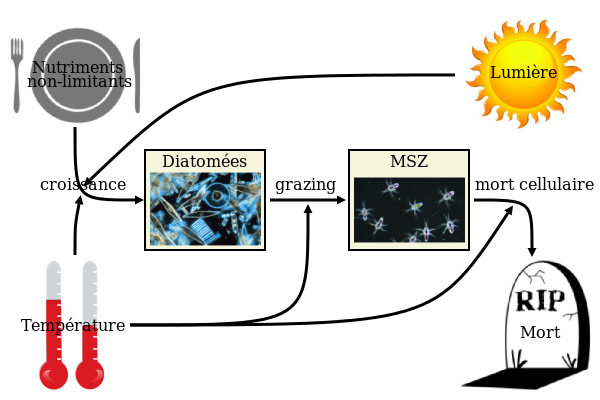
\includegraphics[width=\textwidth]{partie1/diagrammeConceptuel.png}
  \caption{Le modèle conceptuel du système étudié dans le quatrième cours. La croissance du phytoplancton
n'est plus limitée par les nutriments disponibles. Cependant, la croissance est toujours limitée par la
disponibilité de la lumière et de la température. Dans les formules, l'influence de ces deux impacts
environnementals est cachée dans le terme $\mu_{DA}$. Une partie du phytoplancton existant est consommer
par le mésozooplancton (=MSZ). Cette partie est représentée par les fonctions de broutage
différentes fois la concentration du mésozooplancton ($graz_{MSZ}[MSZ]$). Dans le système modèlise
le mésozooplancton n'a pas des prédateurs naturels. Donc, la mort cellulaire naturelle du zooplancton ne peut
plus être négligée (dans les formules c'est le terme $mm_{MSZ}$ qui décrit cette l'influence).
}
  \label{fig:partie1DiagConcept}
\end{figure}

\par{
Pour peut mieux comprendre les équations du modèle, la grille~\ref{tab:partie1signifParam} peut également
être intéressante. Elle donne un aperçu de la signification etc. de chaque terme dans les équations.
}
\par{
Nous voulons encore pointer que les $T_{opt}$ et $d_{opt}$ ont les mêmes valeurs pour les diatomées et le
mésozooplancton simulé. On a donc considerer que les deux espèces sont limitées par la tempèrature
de la même façon.
}

\begin{table}[h!]
\begin{center}
\begin{tabular}{ | c | c | c | c | c | }
\hline
Terme & Signification & Type & Valeur & Unité \\
\hline
$[DA]$ & \pbox{4cm}{Concentration du carbon des diatomées} & Variable d'état & $5$ & ${{mmol C}\over{m^{-3}}}$ \\
$[MSZ]$ & \pbox{4cm}{Concentration du carbon du mésozooplancton}  & Variable d'état & $1$ & ${{mmol C}\over{m^{-3}}}$ \\
$\mu_{DA}$ & \pbox{4cm}{Taux de croissance des diatomées} & \pbox{3cm}{Fonction $\mu_{max}max(T)llum$} & \pbox{4cm}{Dépend de la disponibilité de la lumière (en fonction du $[DA]$) et de la tempèrature} & $Jour^{-1}$ \\
$graz_{MSZ}$ & \pbox{4cm}{Fonction de grazing} & Fonction & \pbox{4cm}{Dépend de la tempèrature et de $[DA]$} & $Jour^{-1}$ \\
$eges_{MSZ}$ & \pbox{4cm}{Taux d'egestion du mésozooplancton} & Paramètre & $0.1$ & $-$ \\
$Y_{MSZ}$ & \pbox{4cm}{Efficience de croissance du mésozooplancton} & Paramètre & $0.25$ & $-$ \\
$mm_{MSZ}$ & \pbox{4cm}{Taux de mortalité du mésozooplancton} & Paramètre & $0.05$ & $Jour^{-1}$ \\
$g_{MSZ}$ & \pbox{4cm}{Taux de grazing maximal} & Paramètre & $1.2$ & $Jour^{-1}$ \\
$max(T)$ & \pbox{4cm}{Fonction de la limitation de la tempèrature} & \pbox{3cm}{Fonction\\(bell-shaped)} & \pbox{4cm}{Dépend de $T, T_{opt}$ et $d_{opt}$} & $-$ \\
$kg_{MSZ}$ & \pbox{4cm}{Constante de grazing} & Paramètre & $10$ & ${{mmol C}\over{m^{-3}}}$ \\
$[DA_0]$ & \pbox{4cm}{Concentration minimale avant le mésozooplancton commencent de consummer les diatomées} & Paramètre & $5$ & ${{mmol C}\over{m^{-3}}}$ \\
$\mu_{max}$ & \pbox{4cm}{Taux de croissance maximal des diatomées} & Paramètre & $1.2$ & $Jour^{-1}$ \\
$T_{opt}$ & \pbox{4cm}{Température optimale (pour les diatomées et du mésozooplancton)} & Paramètre & $16.3$ & $^{\circ}C$ \\
$d_{opt}$ & \pbox{4cm}{Delta T (pour les diatomées et du mésozooplancton)} & Paramètre & $13.7$ & $^{\circ}C$ \\
$T$ & \pbox{4cm}{Température simulée} & Paramètre & $10.0$ & $^{\circ}C$ \\
$llum$ & \pbox{4cm}{Limitation par la lumière} & \pbox{3cm}{Fonction\\$1-e^{-\alpha PAR_Z / \mu_{max}}$} & \pbox{4cm}{Dépend de la lumière disponible, ...} & $-$ \\
\end{tabular}
\end{center}
\end{table}
\clearpage
\begin{table}[h!]
\begin{center}
\begin{tabular}{ | c | c | c | c | c | }
$\alpha$ & \pbox{4cm}{L'efficacité des chloroplastes des diatomées} & Paramètre & $0.02$ & ${mol^{-1}*m^2*sec}\over{quanta * jour}$ \\
$PAR_Z$ & \pbox{4cm}{Lumière disponible par mol chlorophylle} & \pbox{3cm}{Fonction\\$PAR_0*e^{-k_e*z}$} & \pbox{4cm}{Dépend de la latitude, les solides en suspension, ...} & ${mol*quanta}\over{m^2*sec}$ \\
$PAR_0$ & \pbox{4cm}{Lumière solaire incidente} & Paramètre & $23.0$ & ${quanta}\over{m^2*sec}$ \\
$k_e$ & \pbox{4cm}{Coefficient d'extinction verticale de la lumière} & \pbox{3cm}{Fonction\\$0.35+0.02{{1}\over{2}}[DA]$} & \pbox{4cm}{Dépend des solides en suspension, ...} & $^{mol}/_m$ \\
$z$ & \pbox{4cm}{Profondeur de l'habitat} & Paramètre & $1.0$ & $m$ \\
\hline
\end{tabular}
\end{center}
  \caption{Signification, type, valeur et unité de chaque terme/paramètre dans les
équations~\ref{eq:partie1DiffEq1},~\ref{eq:partie1DiffEq2},~\ref{eq:partie1GrazMic},~\ref{eq:partie1GrazMicSeul} et~\ref{eq:partie1GrazHol}.}
  \label{tab:partie1signifParam}
\end{table}
\FloatBarrier

\subsection{Analyse mathèmatique}

\par{
La grille~\ref{tab:partie1etatsStat} donne un aperçu des états stationnaires du système
pour les fonctions de broutage differents. Les constantes supplémentaires utilisées
dans la grille sont définies comme suit:
}
\[
m = mm_{MSZ_{MAX_0}} e ^{- \left ( {{t-t_{opt}}\over{d_{opt}}} \right )}
\]
\[
k = kg_{MSZ}
\]
\[
c = \left ( 1 - eges_{MSZ} \right ) y_{MSZ}
g_{MSZ_{MAX_0}} e ^{- \left ( {{t-t_{opt}}\over{d_{opt}}} \right )}
\]
\[
f = g_{MSZ_{MAX_0}} e ^{- \left ( {{t-t_{opt}}\over{d_{opt}}} \right )}
\]

\begin{table}[h!]
\begin{center}
\begin{tabular}{ | c | c c | }
\hline
fct. de broutage & $[DA]$ & $[MSZ]$ \\
\hline
MIC, MIC\_Seul, HOL & 0 & 0 \\
MIC & $k * {{m}\over{c-m}}$ & ${{\mu_{DA} k \left ( 1 + {{m}\over{c-m}} \right )}\over{f}}$ \\
MIC\_Seuil & ${{m/c*k-m/c[DA_0]+[DA_0]}\over{1-m/c}}$ & ${\mu_{DA} * [DA] * (k + [DA] - [DA_0])}\over{f *([DA] - [DA_0])}$ \\
HOL & $k*\sqrt{{{m}\over{c-m}}}$ & ${{\mu_{DA}k \left ( 1 + {m}\over{c-m} \right )}\over{f \sqrt{{m}\over{c-m}}}}$ \\
\hline
\end{tabular}
\end{center}
  \caption{Les états stationnaires du système pour les fonctions de broutage differents. Les
constantes supplémentaires utilisées ont était définies dans le texte précédent. Les formules sont en accord
avec les simulations informatiques décrites ci-dessous.
}
  \label{tab:partie1etatsStat}
\end{table}
\FloatBarrier

\subsection{Simulation de référence}

\begin{figure}[h!]
  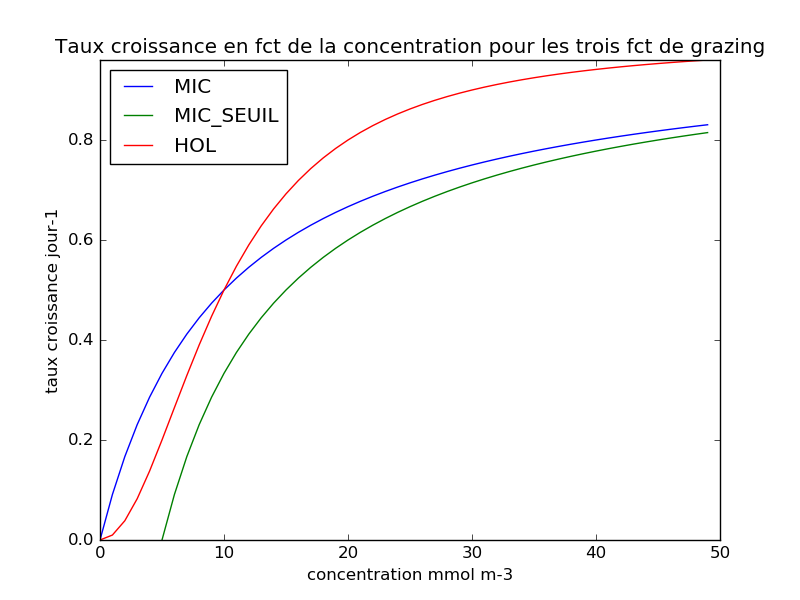
\includegraphics[width=\textwidth]{partie1/grazingFct.png}
  \caption{
La courbe de les trois fonctions~\ref{eq:partie1GrazMic} (MIC),~\ref{eq:partie1GrazMicSeul} (MIC\_SEUIL)
et~\ref{eq:partie1GrazHol} (HOL) en fonction de la concentration $[DA]$.
}
  \label{fig:partie1grazingFcts}
\end{figure}

\begin{figure}[h!]
  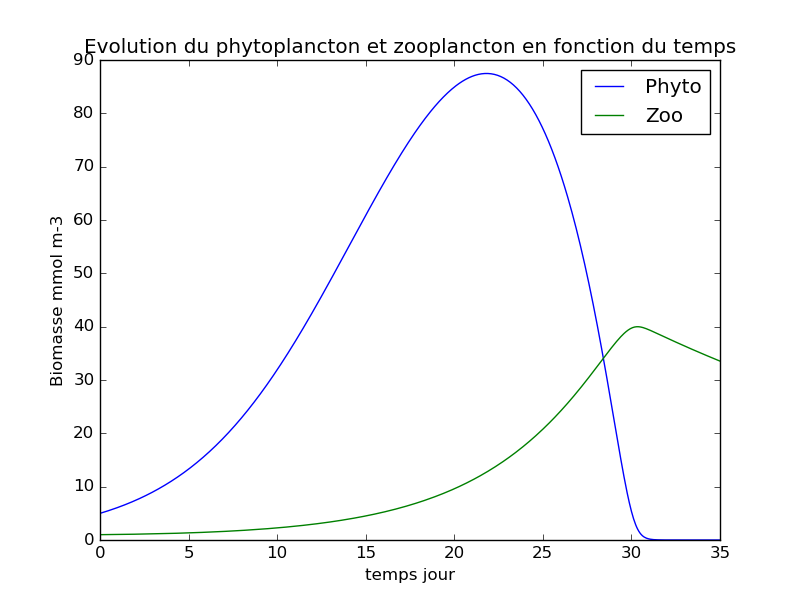
\includegraphics[width=0.5\textwidth]{partie1/refMic35.png}\hfill
  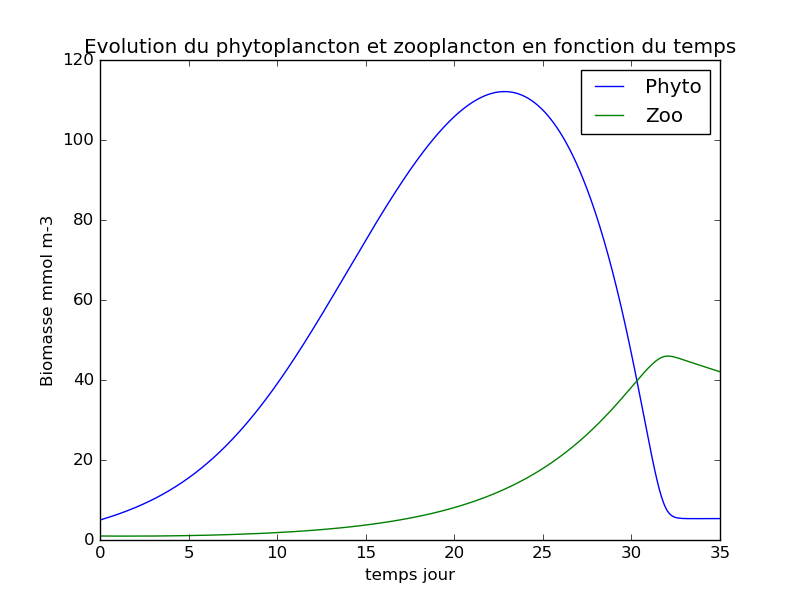
\includegraphics[width=0.5\textwidth]{partie1/refMicSeul35.png}\\
  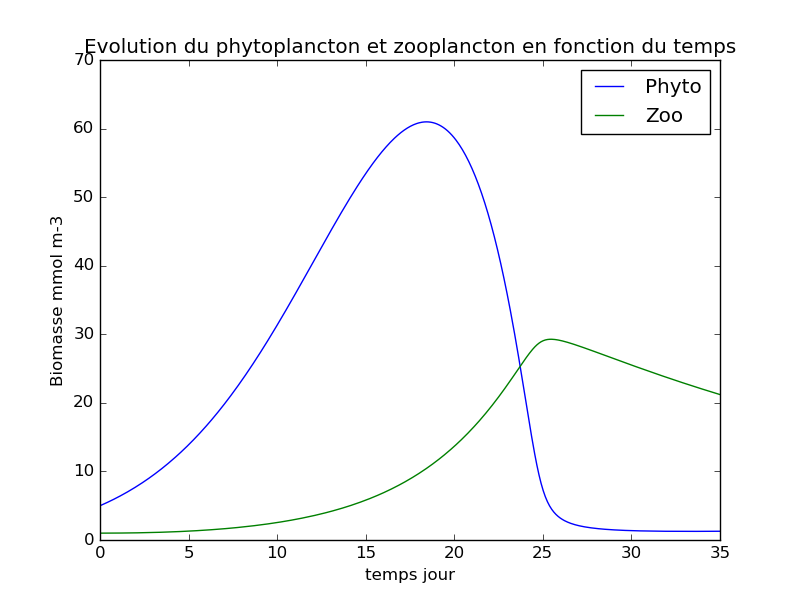
\includegraphics[width=0.5\textwidth]{partie1/refHol35.png}\hfill
  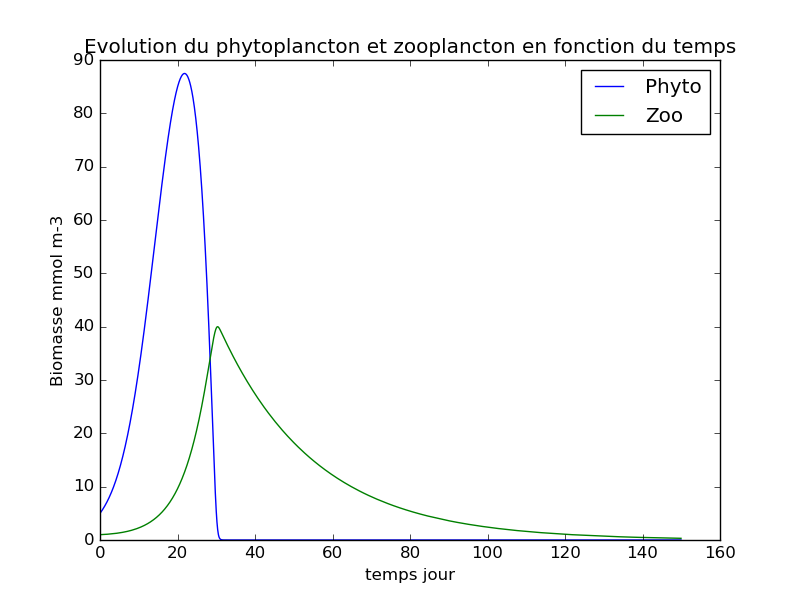
\includegraphics[width=0.5\textwidth]{partie1/refMic150.png}\\
  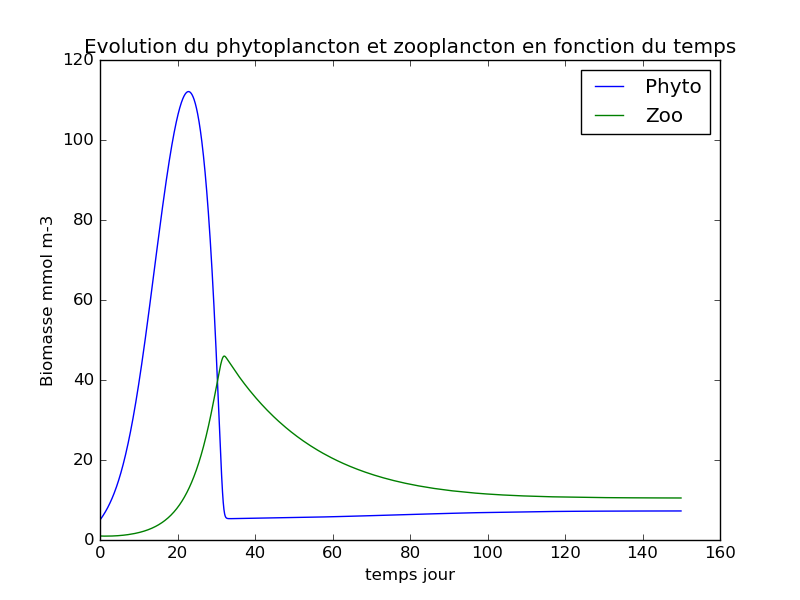
\includegraphics[width=0.5\textwidth]{partie1/refMicSeul150.png}\hfill
  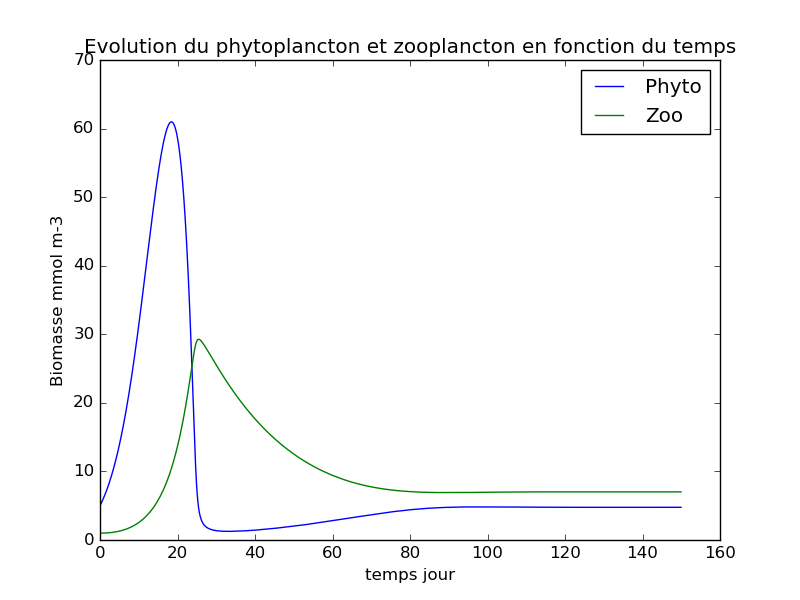
\includegraphics[width=0.5\textwidth]{partie1/refHol150.png}
  \caption{\todo}
  \label{fig:partie1RefSimulations}
\end{figure}

\subsection{Simulation de test 1}


\FloatBarrier
% la deuxième partie
\section{Module de croissance du zooplancton à deux proies}

\subsection{Description du module}

\par{
Dans le quatrième cours on a agrandis le modèle mathématique. On considére maintenant deux espèce de
proies qui sont consommées par le mésozooplancton de façon sélectif ou non-sélectif. Du coup le modèle
conceptuel se changera. On peut admirer le nouveau modèle conceptuel dans la figure~\ref{fig:partie2DiagConc}.
}

\begin{figure}[h!]
  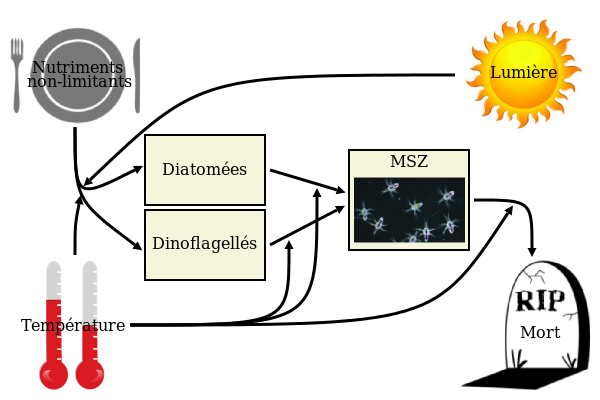
\includegraphics[width=\textwidth]{partie2/diagConc.png}
  \caption{Le modèle conceptuel du système étudié dans le cinquième cours. Par rapport
au modèle conceptuel du quatrième cours (voir figure~\ref{fig:partie1DiagConcept}) on
a augmonter les nombres des espèces (des diatomées et des dinoflagellés) qui peuvent
servir comme proie.
}
  \label{fig:partie2DiagConc}
\end{figure}

\par{
Puisque le diagramme conceptuel était changé on doit revaloriser les équations. Les équations nouveux regardent
comme suit:
}

\begin{equation}
  {{d[DA]}\over{dt}} =
  \mu_{DA} [DA] - graz_{MSZ/DA} [MSZ]
  \label{eq:partie2DiffEq1}
\end{equation}
\begin{equation}
  {{d[DINO]}\over{dt}} =
  \mu_{DINO} [DINO] - graz_{MSZ/DINO} [MSZ]
  \label{eq:partie2DiffEq2}
\end{equation}
\begin{equation}
  {{d[MSZ]}\over{dt}} =
  \left (
    (1- eges_{MSZ}) graz_{MSZ} Y_{MSZ} - mm_{MSZ}
  \right ) [MSZ]
  \label{eq:partie2DiffEq3}
\end{equation}


\begin{equation}
  graz_{MSZ} = graz_{MSZ/DA} + graz_{MSZ/DINO}
  \label{eq:partie2grazMsz}
\end{equation}

\par{
Dans le cas du grazing non sélectif, on considére aussi les équations suivants:
}

\begin{equation}
  [PHYTO] = [DA] + [DINO]
  \label{eq:partie2nonSelEq1}
\end{equation}
\begin{equation}
  graz_{MSZ} = g_{MSZ} max(T) {{[PHYTO]^2}\over{kg_{MSZ}^2 + [PHYTO]^2}}
  \label{eq:partie2nonSelEq2}  
\end{equation}
\begin{equation}
  graz_{MSZ/DA} = graz_{MSZ} {{[DA]}\over{[PHYTO]}}
  \label{eq:partie2nonSelEq2}
\end{equation}
\begin{equation}
  graz_{MSZ/DINO} = graz_{MSZ} {{[DINO]}\over{[PHYTO]}}
  \label{eq:partie2nonSelEq3}
\end{equation}

\par{
Et dans le cas du grazing sélectif, on considére plutôt les équations suivis:
}

\begin{equation}
  graz_{MSZ/DA} = g_{MSZ} max(T) {{\left ( {{[DA]}\over{kg_{MSZ/DA}}}\right )^2}\over
{1 + \left ( {{[DA]}\over{kg_{MSZ/DA}}} \right )^2 + \left ( {{[DINO]}\over{kg_{MSZ/DINO}}} \right )^2}}
  \label{eq:partie2selEq1}
\end{equation}
\begin{equation}
  graz_{MSZ/DINO} = g_{MSZ} max(T) {{\left ( {{[DINO]}\over{kg_{MSZ/DINO}}}\right )^2}\over
{1 + \left ( {{[DA]}\over{kg_{MSZ/DA}}} \right )^2 + \left ( {{[DINO]}\over{kg_{MSZ/DINO}}} \right )^2}}
  \label{eq:partie2selEq2}
\end{equation}
\begin{equation}
  graz_{MSZ} = g_{MSZ/DA} + g_{MSZ/DINO}
  \label{eq:partie2selEq3}
\end{equation}

\par{
Par rapport au travail pratique précendent on peut garder tous les valeurs pour les différents paramètres.
Seulement pour le cas du grazing sélectif, on introduire deux constantes de grazing différentes pour les
deux espèces. Ces constantes ont les valeurs suivantes:
}
\[
kg_{MSZ/DA} = 10 {^{mmol~C}/_{m^3}}
\]
\[
kg_{MSZ/DINO} = 20 {^{mmol~C}/_{m^3}}
\]

\par{
Pour le travail pratique on a du changes les conditions initiales pour les differents tests
(voir tableau~\ref{tab:partie2params}).
}

\begin{table}[h!]
\begin{center}
\begin{tabular}{ | c | c | c | c | c | c | }
\hline
Variable & Référence & Test 1 & Test 2 & Test 3 & Test 4 \\
\hline
DA & $20$ & $30$ & $10$ & $20$ & $20$ \\
DINO & $20$ & $10$ & $30$ & $20$ & $20$ \\
MSZ & $10$ & $10$ & $10$ & $1$ & $20$ \\
\hline
\end{tabular}
\end{center}
  \caption{Les conditions initiales pour en DA, DINO et MSZ pour les differents tests.}
  \label{tab:partie2params}
\end{table}

\clearpage
\subsection{Simulation de référence}

\begin{figure}[h!]
  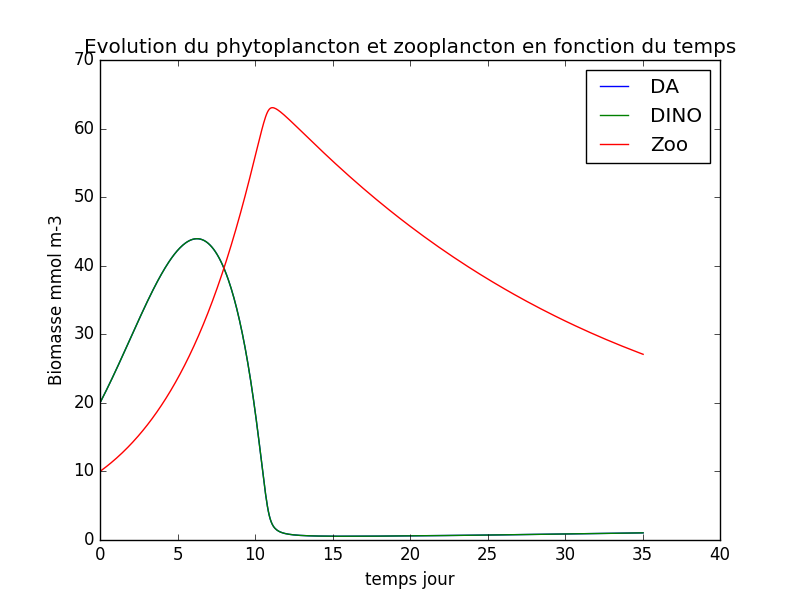
\includegraphics[width=.5\textwidth]{partie2/1Nonselec.png}\hfill
  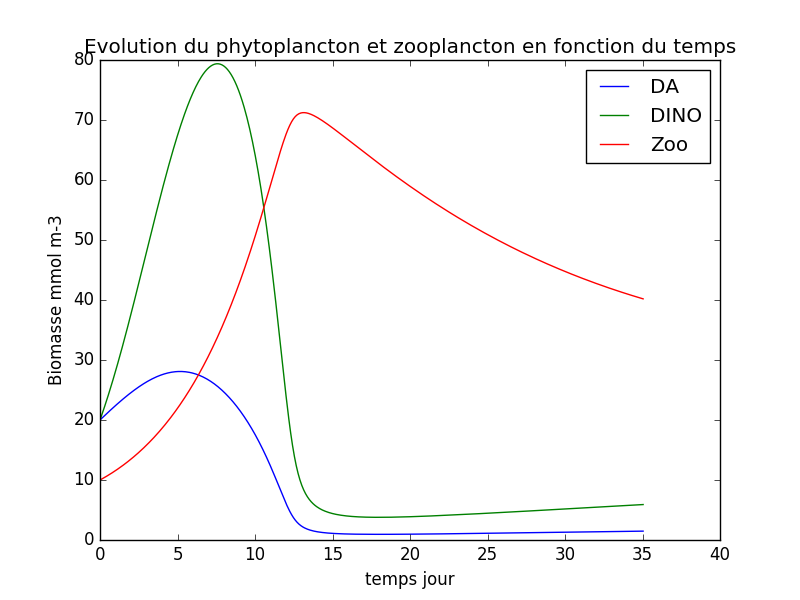
\includegraphics[width=.5\textwidth]{partie2/1Selec.png}
  \caption{Les simulations de référence. Quand on simule le fait que les proies sont mangé par le
mésozooplancton de manière non-sélectif on observe la simulation à gauche. La simulation à droite
est observé pour la fonction de grazing-sélectif.
}
  \label{fig:partie2Ref}
\end{figure}

\par{
Comme on peut voir dans la graphique~\ref{fig:partie2Ref}, 
dans le cas d'un grazing non s\'electif, les deux espèces phytoplanctoniques croissent de la même manière,
ce qui fait que les courbes d'évolution de la biomasse sont confondues. En effet, pour les deux espèces,
tous les paramètres sont égaux, ainsi que les concentrations initiales. Le maximum de biomasse
phytoplanctonique est atteint après 7 jours et a une valeur de 45 ${^{mmol}}/_{m-3}$, tandis que le maximum
de la biomasse zooplanctonique est atteint après 13 jours et a une valeur de 65 ${^{mmol}}/_{m-3}$.
Contrairement au TP précédent, la valeur maximum du zooplancton parait supérieure à celle du phytoplancton.
Cependant, il faut tenir compte du fait que deux populations de phytoplancton sont présentes, et donc que
la concentration maximum de phytoplancton est en fait plus importante que celle du zooplancton.
}
\par{
Dans le cas d'un grazing s\'electif, les deux populations de phytoplancton n'ont ici plus la même évolution.
La concentration maximum des dinoglagellés est atteinte après 7 jours (comme dans le cas non sélectif)
mais a une valeur de 80 ${^{mmol}}/_{m-3}$, tandis que celle des diatomées est atteinte après 5 jours, et a une
valeur de 30 ${^{mmol}}/_{m-3}$. De plus, la concentration maximum du zooplancton est atteinte après 15 jours
et a une valeur de 70 ${^{mmol}}/_{m-3}$.
}
\par{
En effet, les constantes de demi saturation du taux de grazing des deux espèces de phytoplancton sont
ici différentes. Une des espèce a le même que dans le cas du non sélectif (les Diatomées), mais
l'affinité pour les dinoflagellés est plus faible. Ceci fait que les dinoflagellés ont donc la possibilité
d'atteindre une concentration maximum plus importante, et que les diatomées ont une concentration maximum
plus faible.
}
\par{
De plus, on peut voir que la décroissance des dinoflagellés est beaucoup plus rapide que celle des
diatomées. En effet, au jour 6, la concentration en dinoflagellés est très importante et celle en
diatomées est faible. Or, on peut voir dans l'équation du taux de grazing (équation~\ref{eq:partie2selEq2})
du dinoflagellé que si la concentration en dinoflagellés est grande et que la concentration en diatomées
est faible, alors le taux de grazing des dinoflagellés est grand. Ceci explique la décroissance
rapide des dinoflagellés. A l'inverse, si on regarde l'équation du taux de grazing des diatomées
(équation), si la concentration en dinoflagellés est grande et que la concentration en diatomées
est faible, alors plus le taux de grazing des diatomées est faible. Ainsi, la population de diatomée a
une décroissance beaucoup plus lente.
}
\par{
De plus, on voit que les concentrations minimales ne sont pas les mêmes. En effet, le zooplancton a la
capacité d'utiliser plus efficacement les Diatomées à faible concentration que les dinoflagellés,
c'est pourquoi la concentration minimum en Diatomée est plus faible.
}

\subsection{Tests de la sensitivité}

\begin{figure}[h!]
  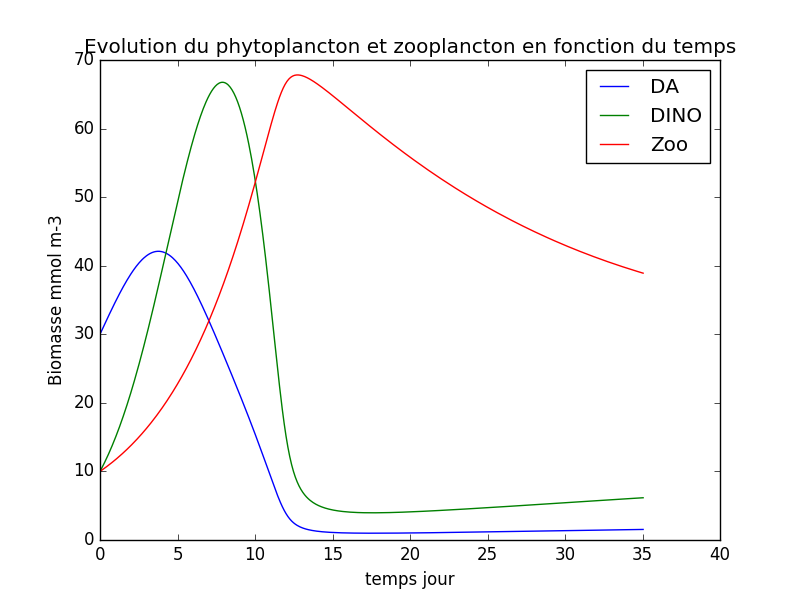
\includegraphics[width=.5\textwidth]{partie2/test1sel.png}\hfill
  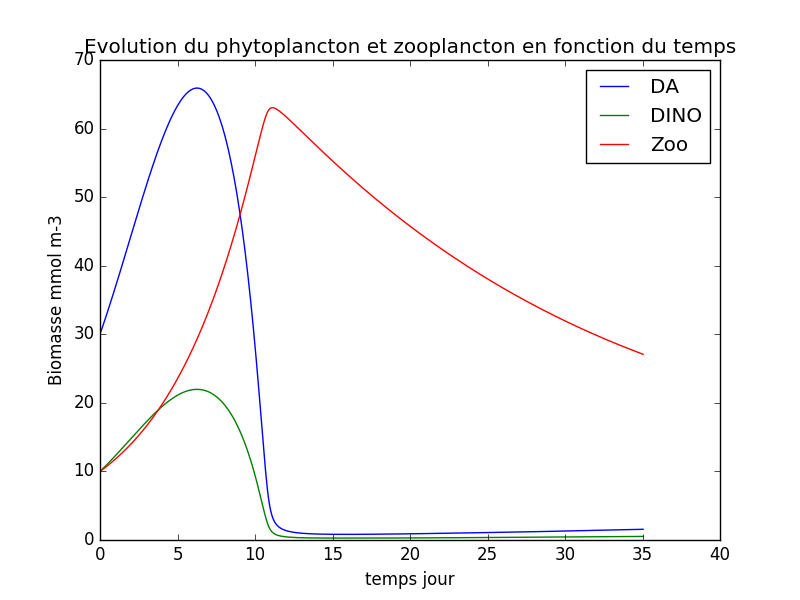
\includegraphics[width=.5\textwidth]{partie2/test1nonsel.png}\\
  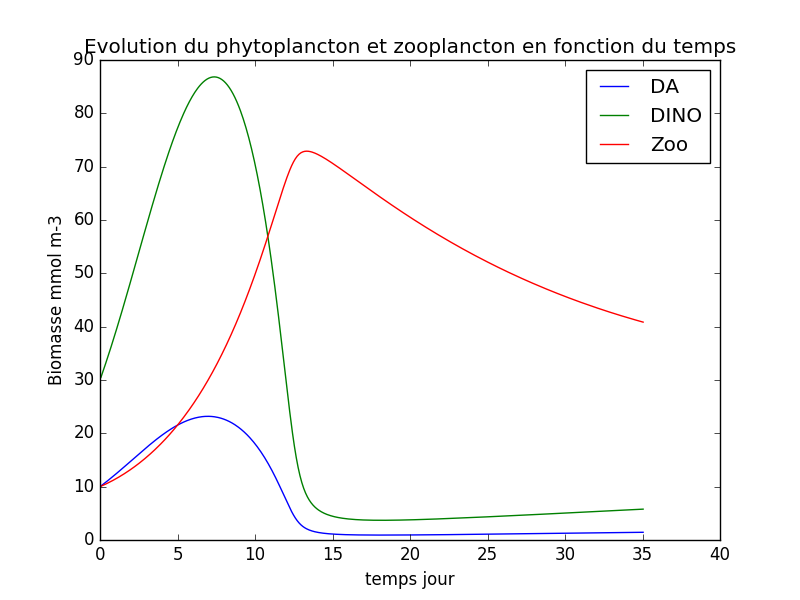
\includegraphics[width=.5\textwidth]{partie2/test2sel.png}\hfill
  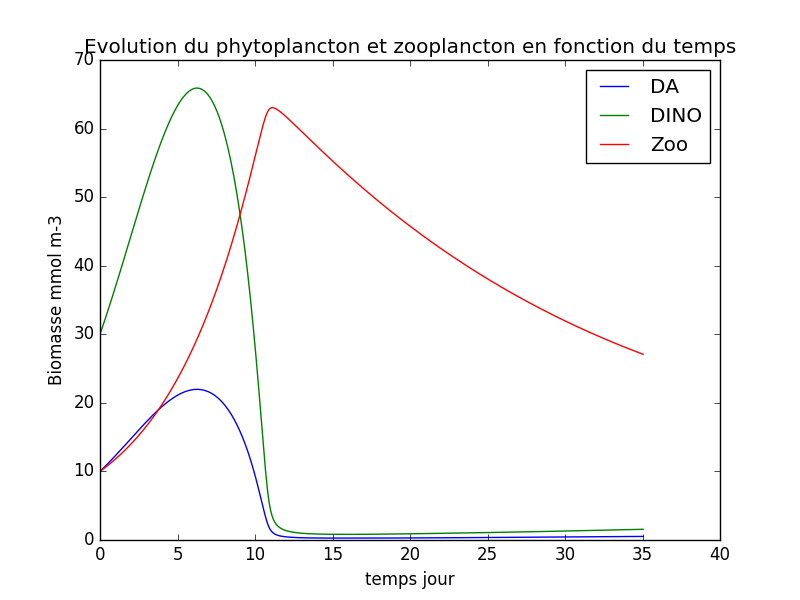
\includegraphics[width=.5\textwidth]{partie2/test2nonsel.png}
  \caption{Cettes simulations montrent l'impact d'une changement des conditions initiales sur
les traces de concentration pour les différentes espèces. On observe les simulations à gauche
quand on simule le fait que les proies sont mangé par le mésozooplancton de manière sélectif.
(Et logiquement on obtient les simulations à droite en outilisent la fonction non-sélectif.)
La première ligne montre le test 1 et la deuxième ligne le test 2 (cmp
tableau~\ref{tab:partie2params}).}
  \label{fig:partie2Test1}
\end{figure}

\subsection{Test 1 - cas sélectif}
\par{
On discute d'abords le cas du prèmiere test avec la fonction de grazing non-sélectif (voir
figure~\ref{fig:partie2Test1}, première ligne droite). Ici, bien que les constantes de demi saturation des
taux de grazing soient
les mêmes, les concentrations initiales en diatomées et dinoflagellés sont différentes. Ainsi, puisque
la concentration en diatomées est diminuée de 10 ${^{mmol}}/_{m-3}$ mais que la concentration en
dinoflagellés est augmentée
de 10 ${^{mmol}}/_{m-3}$, et que les deux populations de phytoplancton ont exactement les mêmes paramètres,
l'évolution du zooplancton est exactement la même que dans le cas de la référence. Cependant, les diatomées
atteignent une concentration maximum beaucoup plus élevée que dans le cas de la référence
(65 ${^{mmol}}/_{m-3}$), tandis que la concentration maximum des Dinoflagellés est plus faible
(20 ${^{mmol}}/_{m-3}$). La somme des concentrations du phytoplancton est exactement la même que dans
le cas de la référence, puisqu'une fois de plus, les deux populations de phytoplancton ont exactement
les mêmes paramètres.
}
\subsection{Test 1 - cas non-sélectif}
\par{
Pour comparer, dans le cas du première test avec la fonction de grazing sélectif (voir
figure~\ref{fig:partie2Test1}, première ligne gauche), on observe une autre simulation.
Dans cette simulation, l'affinité pour les Dinoflagellés est plus faible que pour les diatomées.
Cependant, la concentration initiale en dinoflagellés est plus faible que dans le cas de la référence,
ce qui explique que la concentration maximum en dinoflagellés atteinte est plus faible que dans le cas
de la référence.
}
\par{
De la même manière, l'affinité pour les diatomées est plus grande, mais la concentration initiale en
diatomées est plus grande, ce qui explique que la concentration maximum en diatomées est plus élevée
que dans le cas de la référence.
}
\par{
De plus, puisque l'affinité pour les diatomées est plus grande et que la concentration initiale en
diatomées est plus grande, le maximum de biomasse est atteint plus rapidement. 
}
\par{
La concentration maximum en zooplancton est cependant plus faible que dans le cas de la référence.
Ainsi, augmenter la concentration initiale de la proie préférée entraîne une diminution du maximum
du zooplancton. 
}

\subsection{Test 2 - cas non-sélectif}
\par{
Comme on peut voir dans la deuxième ligne droite de la figure~\ref{fig:partie2Test1}, pour cette simulation
la concentration initiale des dinoflagellés a été augmentée de 10 ${^{mmol}}/_{m-3}$, tandis que la
concentration initiale des diatomées a été diminuée de 10 ${^{mmol}}/_{m-3}$. Ici aussi, tous les
paramètres des deux populations de phytoplancton sont les mêmes. Ainsi, la concentration maximum
en dinoflagellés est plus importante que dans le cas de la référence, et la concentration maximum en
diatomées est plus faible. Cependant, la somme des deux concentrations des deux populations de phytoplancton
est la même que dans le cas de la référence, et ainsi, l'évolution du zooplancton l'est aussi.
}
\subsection{Test 2 - cas sélectif}
\par{
La concentration initiale en dinoflagellés, qui sont moins appréciés que les diatomées, est plus grande
que dans le cas de la référence. Inversement, la concentration initiale des diatomées est plus faible.
Ainsi, cette situation mène à un taux de grazing des diatomées faible, comme on peut le remarquer dans
l'équation~\ref{eq:partie2selEq1}, et à un taux de grazing des dinoflagellés élevé, comme on peut le
remarquer dans l'équation~\ref{eq:partie2selEq2}. Ceci permet aux diatomées de croître sur une plus
longue période, et d'atteindre un maximum de biomasse relativement plus grand que dans le cas de la
référence. Inversement, la population de dinoflagellés atteint un maximum relativement plus faible,
et atteint ce maximum plus tôt que dans le cas de la référence. De plus, on peut voir que diminuer
la concentration de la proie la plus appréciée entraîne une augmentation du maximum de concentration
du zooplancton.
}

\begin{figure}
  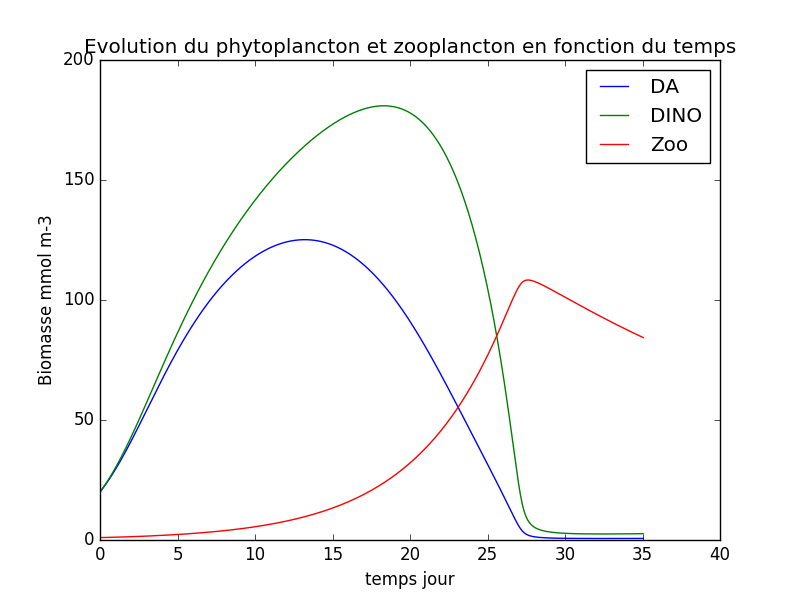
\includegraphics[width=.5\textwidth]{partie2/test3sel.png}\hfill
  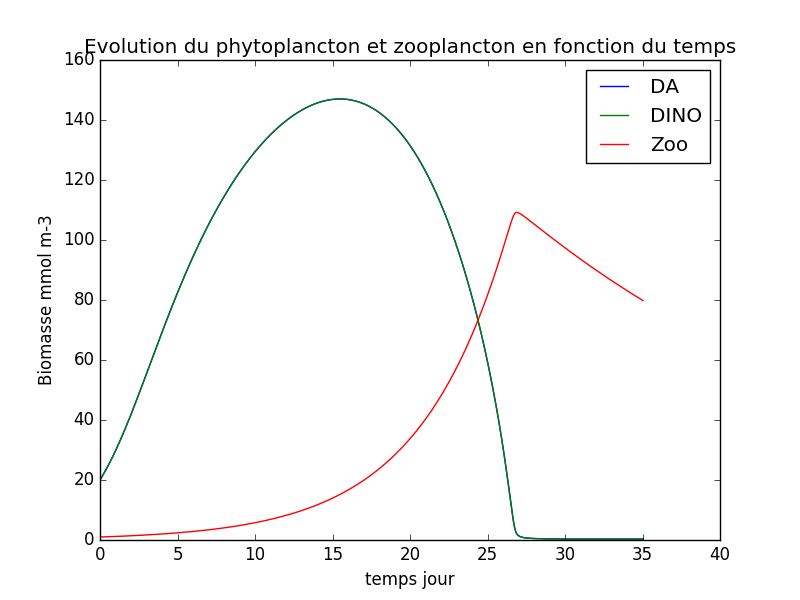
\includegraphics[width=.5\textwidth]{partie2/test3nonsel.png}\\
  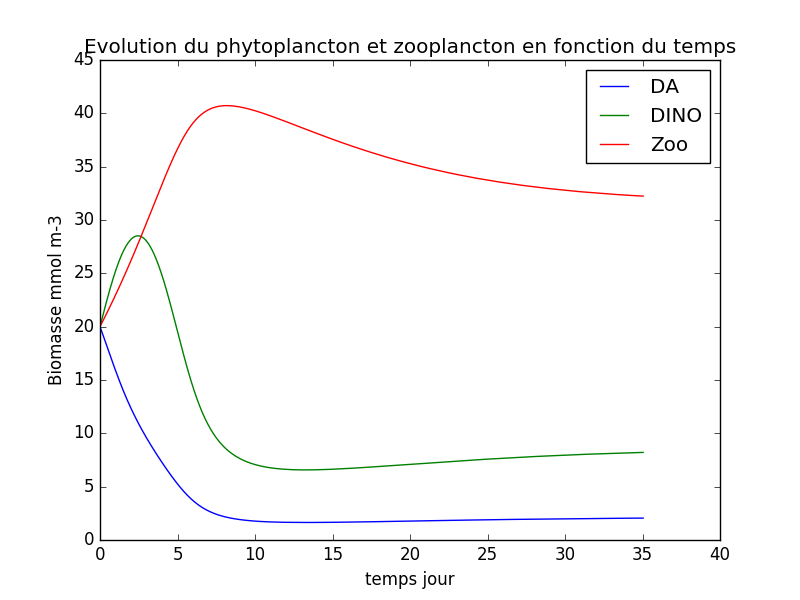
\includegraphics[width=.5\textwidth]{partie2/test4sel.png}\hfill
  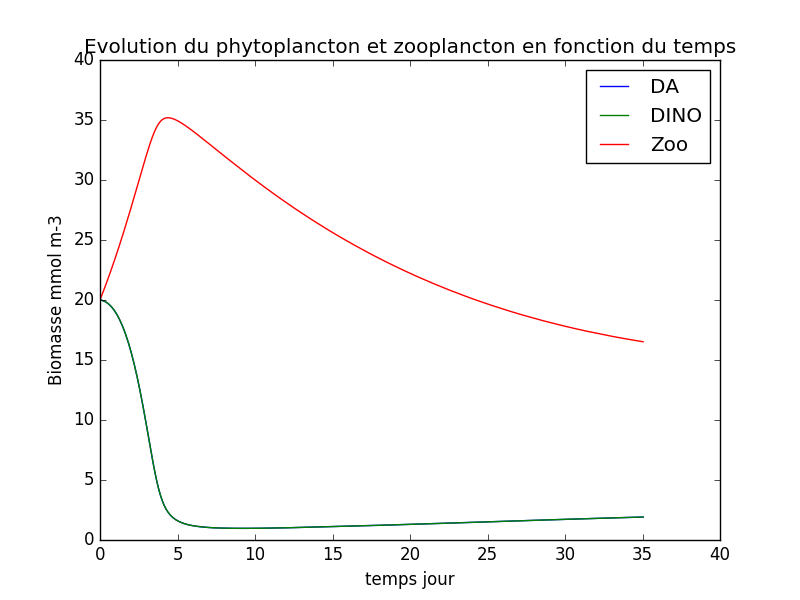
\includegraphics[width=.5\textwidth]{partie2/test4nonsel.png}
  \caption{Cettes simulations montrent l'impact d'une changement des conditions initiales sur
les traces de concentration pour les différentes espèces. On observe les simulations à gauche
quand on simule le fait que les proies sont mangé par le mésozooplancton de manière sélectif.
(Et logiquement on obtient les simulations à droite en outilisent la fonction non-sélectif.)
La première ligne montre le test 3 et la deuxième ligne le test 4 (cmp
tableau~\ref{tab:partie2params}).}
  \label{fig:partie2Test2}
\end{figure}

\subsection{Test 3 - cas non-sélectif}
\par{
Commen on peut observer dans la figure~\ref{fig:partie2Test2},
les concentrations initiales ainsi que tous les paramètres sont les mêmes pour les deux espèces
de phytoplancton. Cependant, la concentration initiale en zooplancton est 10 fois plus faible que
dans le cas de la référence. Ainsi, les deux espèces de phytoplancton croissent pendant une plus longue
période, et atteignent donc un maximum de biomasse plus important. Puisque ces populations de
phytoplancton atteignent un maximum de biomasse plus tard, alors le zooplancton atteint aussi le sien
plus tard, et celui-ci est donc plus grand. 
}

\subsection{Test 3 - cas sélectif}
\par{
Dans cette simulation (voir figure~\ref{fig:partie2Test2}, première ligne gauche), la concentration initiale
en zooplancton est 10 fois inférieure que dans le cas
de la référence. Ceci permet aux deux populations de phytoplancton de croître plus longtemps et donc
d'atteindre des maxima de concentration plus grands. Ainsi, la population de zooplancton peut aussi
croître plus longtemps et donc atteindre une concentration maximum plus grande. De plus, les diatomées
étant l'espèce la plus appréciée par le zooplancton, celle-ci atteindra son maximum avant les dinoflagellés.
}

\subsection{Test 4 - cas non-sélectif}
\par{
Dans cette simulation (voir figure~\ref{fig:partie2Test2}, deuxième ligne droite), la concentration initiale
en zooplancton est doublée par rapport à la référence.
Ainsi, la pression de grazing est telle qu'elle empêche toute croissance des deux populations de phytoplancton.
En effet, cette concentration initiale importante fait que le terme de mortalité des deux espèces
phytoplanctoniques est toujours supérieur au terme de croissance (voir equations~\ref{eq:partie2DiffEq1}
et~\ref{eq:partie2DiffEq2}).
}

\subsection{Test 4 - cas sélectif}
\par{
De la même manière que dans la simulation précédente, la concentration initiale du zooplancton
est tellement grande qu'elle empêche la croissance des Diatomées, qui sont les proies préférées.
En effet, le terme de croissance est toujours inférieur au terme de mortalité, dans l'équation de
l'évolution des Diatomées. Cependant, la population de Dinoflagellés peut quand même croître, car
le zooplancton a une affinité plus faible pour ceux-ci.
}

\subsection{Conclusion}

Nous pouvons constater que dans le cas d'un grazing non sélectif, si nous modifions les concentrations initiales des populations de phytoplancton, mais que la somme de ces concentrations restent les mêmes, alors l'évolution du zooplancton reste la même. Si nous gardons les mêmes conditions initiales pour les deux populations de phytoplancton, alors les deux populations vont suivre exactement la même évolution. Cela est du au fait que tous les paramètres, pour les deux populations de phytoplancton, sont les mêmes. En réalité, même si le grazing du zooplancton n'est pas sélectif, nous devrions observer des différences entre les évolutions des populations de phytoplancton.
De plus, nous pouvons constater que le zooplancton a toujours une concentration plus grande quand le grazing est sélectif que quand il est non sélectif. En effet, dans le cas sélectif, nous avons diminué l'affinité du zooplancton pour une des espèces, par rapport au cas non sélectif. Si nous avions augmenté l'affinité pour une des espèces, nous aurions observé une tendance totalement inverse.

\FloatBarrier
% conclusion
\section{Conclusion}

\FloatBarrier

\end{document}
